\documentclass[10pt]{beamer}

\usetheme{Warsaw}
\beamertemplatenavigationsymbolsempty

\usepackage[utf8x]{inputenc}
\usepackage[francais]{babel}
\usepackage{hyperref}
\usepackage{amsmath}
\usepackage{graphicx}
\usepackage{tikz}
\usepackage{multicol}
\usetikzlibrary{automata,positioning}
\graphicspath{{./img/}}
\DeclareGraphicsExtensions{.png, .jpeg, .jpg}


\renewcommand*\thesection{\arabic{section}}


\AtBeginSection[]{%
  \begin{frame}<beamer>
    \frametitle{Plan}
    \tableofcontents[sectionstyle=show/hide,subsectionstyle=hide/show/hide]
  \end{frame}
  \addtocounter{framenumber}{-1}
}



\title{Obtention efficace des Longest Common Prefixes}
\author{Rémi Bois, Loïc Jankowiak}
\date{\today}

\begin{document}

\begin{frame}
  \maketitle

\end{frame}

\begin{frame}
  \tableofcontents
\end{frame}

\section{Contexte}
\label{sec:context}


\begin{frame}
  \frametitle{Recherche de motif à partir d'un tableau des suffixes
    et des longest common prefixes}
  %description de l'efficacité de la recherche via le tableau des
  %suffixes en termes de complexité algorithmique et spaciale

  \begin{block}{arbre des suffixes vs tableau des suffixes} 
    Le tableau des suffixes est une représentation compacte de l'arbre
    des suffixes. Le principal avantage du tableau des suffixes comparé à
    l'arbre des suffixes est la place mémoire occupée, environ 4 fois
    moins importante. Cette contrainte est importante lors de
    recherches sur de longs textes, notamment en bioinformatique \cite{Raffinot11}.
  \end{block}

  \pause

  \begin{block}{La recherche de motifs}
    Le tableau des suffixes permet de trouver les occurrences d'un
    motif dans un texte en $O(m*log(n))$. Associé aux informations sur
    les plus longs préfixes communs (Longest Common Prefixes,
    \emph{lcp}), il permet une recherche en $O(m + log(n))$ \cite{Manber93}.
  \end{block}
  
\end{frame}

\begin{frame}
  \frametitle{Un élément manquant : les longest common prefixes}
  %cadre dans lequel on se place : on a le texte et le tableau des
  %suffixes. Il manque les lcp pour faire une recherche efficace

  \begin{block}{Les lcps pendant la construction}
      Dans les faits, le calcul des lcp se fait lors de la construction de
      l'arbre des suffixes, ou du tableau des suffixes. Il ne rajoute pas
      de complexité à ces constructions (l'ordre de grandeur reste
      identique).
  \end{block}
  \pause
  \begin{block}{Les lcps après la construction}
    L'article présenté propose un moyen efficace d'obtenir
    les informations des lcp lorsque celles-ci ne sont pas
    disponibles\cite{Kasai01}.
  \end{block}

\end{frame}


\begin{frame}
  \frametitle{Un contexte réaliste ?}
  %intro sur les deux problèmes qu'on explorera plus tard
  
  \begin{block}{Une application concrète}
    Un algorithme de compression basé sur la transformation de
    Burrow-Wheeler \cite{Burrows94}, très utilisé (\emph{bizp2}), permet
    de retrouver, lors de la décompression, le tableau des suffixes. 
    
    Il ne manque alors plus que les informations sur les lcps pour faire
    une recherche efficace. 
  \end{block}

\end{frame}

\section{Calculer les lcps en O(n)}
\label{sec:algo}

%Faut voir comment on organise ça. Faut le faire tourner sur un
%exemple (abraca ?)

\begin{frame}
  \frametitle{Quelques notations}

  Le calcul des \textit{lcp} utilise les notations suivantes~:
  \begin{itemize}
  \item \textit{lcp} : Longest Common Prefixes
  \item \textit{A} : Un texte
  \item \textit{Pos} : le tableau des suffixes de A trié par ordre
    lexicographique. 
  \item \textit{Rank} : le tableau inverse de \textit{Pos}.
  \item \textit{Height} : le tableau des \textit{lcp}. Il correspond à la
    hauteur du plus petit ancêtre commun de deux feuilles consécutives dans
    l'arbre des suffixes~:
    \begin{center}
    $\mathit{Height}[i] = \mathit{lcp}(\mathit{Pos}[i-1], \mathit{Pos}[i])$
    \end{center}
  \end{itemize}
  \hfill \\ \hfill \\ \hfill \\

  L'idée est d'itérer sur les suffixes triés par indice de début, et de
  calculer les \textit{lcp} sur des suffixes adjacents dans \textit{Pos}.
\end{frame}

\begin{frame}
  \frametitle{Algorithme GetHeight}

  \begin{block}{Propriété 1}
  Le \textit{lcp} de deux sous-chaînes est le minimum des \textit{lcp} de
  toutes les sous-chaînes adjacentes dans l'intervalle du tableau Pos.
  \end{block}
  \begin{block}{Propriété 2}
  Lorsque l'on supprime le premier caractère du suffixe (ie. lorsque l'on
  avance d'un caractère), l'ordre des suffixes comparés est conservé dans
  \textit{Pos}.
  \end{block}
\end{frame}

\begin{frame}

  \frametitle{Algorithme GetHeight}
  
  
  \begin{block}{Propriété 3}
    Lorsque l'on avance d'un caractère, le \textit{lcp} diminue de 1
    si le lcp précédent était $\geq$ 1. 
  \end{block}
  
  \pause

  \begin{columns}
    \begin{column}{.48\textwidth}
      
      Aucun caractère ne diffère :
      
      aaaaa\$

      aaaa\$

      $\hookrightarrow$ lcp = 4

      aaaa\$

      aaa\$

      $\hookrightarrow$ lcp = 3

      
      Le lcp diminue de 1 à chaque fois qu'on passe au suffixe suivant.
      
      % Left Part
    \end{column}%
    \hfill%
    \pause
    \begin{column}{.48\textwidth}
        
      Au moins un caractère diffère (mais lcp $>$ 1):
      
        aabaa\$

        abaa\$

        $\hookrightarrow$ lcp = 1

        abaa\$

        baa\$

        $\hookrightarrow$ lcp = 0
        
        Le lcp diminue de 1 à chaque fois qu'on passe au suffixe suivant.
        
      \end{column}%
      \end{columns}
  
\end{frame}

\begin{frame}
  \frametitle{Pourquoi calculer \textit{Height[q]} à partir de
    \textit{Height[p]}~?}

  On pose $p = \mathit{Rank}[i-1]$ et $q = \mathit{Rank}[i]$.
  \begin{block}{Théorème}
  Si $\mathit{Height}[p] > 1$, alors~:
  $\mathit{Height}[q] ≥ \mathit{Height}[p] - 1$
  \end{block}
  \begin{block}{Preuve}

  \end{block}
\end{frame}


\begin{frame}
  \frametitle{Algorithme GetHeight}
  \scriptsize
  \begin{multicols}{2}
GetHeight\\
Entrée: Une chaîne A et son tableau des suffixes\\ \hfill \\
\begin{tabular}{|l}
  \verb!pour i de 1 à n faire!\\
  \verb! ~Rank[Pos[i]] ← i!\\
  \verb!fin pour!\\
  \verb!h ← 0!\\
  \verb!pour i de 1 à n faire!\\
  \verb! ~si Rank[i] > 1 alors!\\
  \verb! ~ ~k ← Pos[Rank[i]-1]!\\
  \verb! ~ ~tantque A[i+h] = A[k+h] faire!\\
  \verb! ~ ~ ~h ← h+1!\\
  \verb! ~ ~fin tq!\\
  \verb! ~ ~Height[Rank[i]] ← h!\\
  \verb! ~ ~si h > 0 alors h ← h-1 fin si!\\
  \verb! ~fin si!\\
  \verb!fin pour!\\
\end{tabular}\\
  \columnbreak
  \begin{tabular}{ll}
    $i$      & \verb!12345678!\\
    \hline
    chaîne & \verb!atalata\$!\\
    \texttt{Pos}    & \texttt{31574268}\\
    \texttt{Rank}   & \texttt{26153748}\\
    \texttt{Height} & \only<1>{\texttt{.1......}
                      }\only<2-3>{\texttt{.1...0..}
                      }\only<4>{\texttt{.1..00..}
                      }\only<5>{\texttt{.13.00..}
                      }\only<6>{\texttt{.1310020}}\\
  \end{tabular}\\
  \hfill \\
  h ← 0\\
  i = 1, Rank[1] = 2 $>$ 1\\
  ~ ~ j ← Pos[1] = 3\\
  ~ ~ ~ A[1] = A[3] ? Oui $\Rightarrow$ h ← 1\\
  ~ ~ ~ A[2] = A[4] ? Non $\Rightarrow$ Height[2] ← 1\\
  ~ ~ ~ h ← 0\\
  \pause
  i = 2, Rank[2] = 6 $>$ 1\\
  ~ ~ j ← Pos[5] = 4\\
  ~ ~ ~ A[2] = A[4] ? Non $\Rightarrow$ Height[6] ← 0\\
  \pause
  i = 3, Rank[3] = 1\\
  \pause
  i = 4, Rank[4] = 5 $>$ 1\\
  ~ ~ j ← Pos[4] = 7\\
  ~ ~ ~ A[4] = A[7] ? Non $\Rightarrow$ Height[5] ← 0\\
  \pause
  i = 5, Rank[5] = 3 $>$ 1\\
  ~ ~ j ← Pos[3-1] = Pos[2] = 1\\
  ~ ~ ~ A[5] = A[1] ? Oui $\Rightarrow$ h ← 1\\
  ~ ~ ~ A[6] = A[2] ? Oui $\Rightarrow$ h ← 2\\
  ~ ~ ~ A[7] = A[3] ? Oui $\Rightarrow$ h ← 3\\
  ~ ~ ~ A[8] = A[4] ? Non $\Rightarrow$ Height[3] ← 3\\
  ~ ~ ~ h ← 2\\
  \pause
  \ldots

  \end{multicols}
  \normalsize
\end{frame}


\section{Application à la recherche de motif dans un texte compressé}
\label{sec:appcompress}

\begin{frame}
  \frametitle{La compression par Block-Sorting}
  %complexité, implémentations

  \begin{block}{Un bon compromis}
    Block-sorting parvient à obtenir un très bon taux de compression
    tout en étant rapide (vitesse proche de LZ et compression proche
    des modèles statistiques\cite{Burrows94}).
  \end{block}

  \begin{block}{Basée sur une idée ``simple''}
    Le but est de rapprocher les caractères identiques d'un texte et
    d'utiliser un encodage ``move-to-front'' consistant à indiquer la
    distance du prochain caractère identique. On utilise ensuite un
    codage de Huffman pour encoder la suite obtenue.
  \end{block}


\end{frame}

\begin{frame}
  \frametitle{Comment ça marche ?}
  %exemple sur abcabbca$. On s'arrête après la rotation et l'obtention de
  %L, I. On explique "grossièrement" la suite (en une dizaine de
  %secondes)
  \begin{figure}
    
\includegraphics[width=0.22\textwidth]{start_burrows}
  \end{figure}

\end{frame}

\begin{frame}
  \frametitle{Comment ça marche ?}
  %exemple sur abcabbca$. On s'arrête après la rotation et l'obtention de
  %L, I. On explique "grossièrement" la suite (en une dizaine de
  %secondes)
  \begin{figure}
    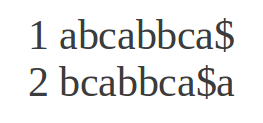
\includegraphics[width=0.21\textwidth]{1_burrows}
  \end{figure}

\end{frame}

\begin{frame}
  \frametitle{Comment ça marche ?}
  %exemple sur abcabbca$. On s'arrête après la rotation et l'obtention de
  %L, I. On explique "grossièrement" la suite (en une dizaine de
  %secondes)
  \begin{figure}
    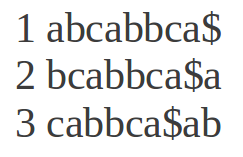
\includegraphics[width=0.2\textwidth]{2_burrows}
  \end{figure}

\end{frame}

\begin{frame}
  \frametitle{Comment ça marche ?}
  %exemple sur abcabbca$. On s'arrête après la rotation et l'obtention de
  %L, I. On explique "grossièrement" la suite (en une dizaine de
  %secondes)
  \begin{figure}
    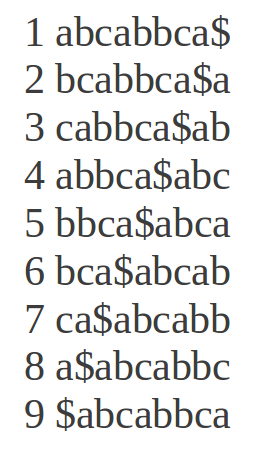
\includegraphics[width=0.2\textwidth]{3_burrows}
  \end{figure}

\end{frame}

\begin{frame}
  \frametitle{Comment ça marche ?}
  %exemple sur abcabbca$. On s'arrête après la rotation et l'obtention de
  %L, I. On explique "grossièrement" la suite (en une dizaine de
  %secondes)
  \begin{figure}
    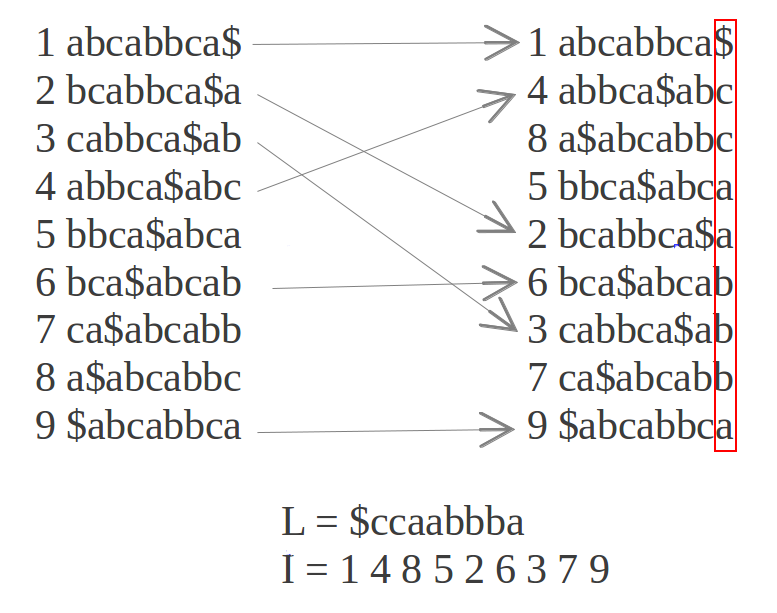
\includegraphics[width=0.5\textwidth]{full_burrows}
  \end{figure}

\end{frame}

\begin{frame}
  \frametitle{Pourquoi ça nous intéresse ?}
  %on peut retrouver le tableau des suffixes à partir de L, I mais il
  %nous manque les informations sur les LCPs. On peut les retrouver en
  %O(n).

  \begin{block}{Comme un air de famille entre I et Pos}
    Le tableau I est en fait le tableau des suffixes.
    Il ne manque donc plus que les informations sur les lcp pour faire
    une recherche efficace.
  \end{block}

\end{frame}

%Une conclusion à cette section ?


% \section{Simulation d'un parcours bottom-up de l'arbre des suffixes}
% \label{sec:appbottomup}

%Aucune idée pour l'instant. Pas sûr qu'on aura le temps de présenter
%en détail cette section.

\section{Conclusion}
\label{sec:conclusion}

\begin{frame}
  \frametitle{Un algorithme performant et simple}
  %rappel de la complexité, des cas d'utilisations, ...

  \begin{block}{Complexité}
    \begin{itemize}
    \item Un tableau de taille n-1 à stocker (même ordre de grandeur que les
      tableaux de lcp classiques)
    \item Un espace mémoire de $13n $ lors du calcul (peut être réduit à $9n$ \cite{Manzini04})
    \item Un calcul en O(n)
    \end{itemize}
  \end{block}

  \pause

  \begin{block}{Des applications concrètes}
    \begin{itemize}
    \item Recherche après décompression d'un texte sous Burrows-Wheeler
    \item Peut simuler un parcours bottom-up de l'arbre des suffixes
    \end{itemize}
  \end{block}

  \pause

  \begin{block}{Une structure extensible}
    Abouelhoda et al\cite{Abouelhoda200453} ont proposé d'améliorer la structure obtenue par
    un arbre d'intervalles des lcps qui permet d'obtenir la liste des
    enfants d'un noeud interne à l'arbre.
  \end{block}

\end{frame}

\begin{frame}
  \frametitle{Des questions ?}
  %une image sympa

\begin{tikzpicture}[shorten >=1pt,node distance=2cm,on grid,auto] 
   \node[state,initial] (q_0)   {$q_0$}; 
   \node[state] (q_1) [above right=of q_0] {$q_1$}; 
   \node[state] (q_2) [below right=of q_0] {$q_2$}; 
   \node[state] (q_5) [right=3cm of q_0]{$q_5$};
   \node[state] (q_6) [right=2.5cm of q_5]{$q_6$};
   \node[state,accepting](q_7) [right=3cm of q_6] {$q_7$};
    \path[->] 
    (q_0) edge  node {Avez} (q_1)
    edge  node [swap] {Posez} (q_2)
    (q_1) edge node {vous} (q_5)
    (q_2) edge node [swap] {nous} (q_5)
    (q_5) edge node {des} (q_6)
    (q_6) edge node {questions} (q_7);
\end{tikzpicture}


\end{frame}

\begin{frame}[allowframebreaks]
  \frametitle{Références}
  %les articles cités
  \bibliographystyle{amsalpha}
  \small
  \bibliography{./pres.bib}
\end{frame}

\end{document}